\chapter{Evaluation} 
\label{cha:evaluation}
Following the model strategy defined in the previous chapter, all model learning and evaluation scripts were run on a computing cluster, the \gls{pc2}.
Several \glspl{pso} were conducted, each with a different target to optimize for.
During every swarm iteration, computational requirements for each model and its hyper-parameters are set heuristically according to those parameters having a significant impact on the optimal training time and on allocatable resources.
The neural network framework Chainer comes with a built-in parallelization mechanism on CPU and GPU level and hence the only challenge here is to find the optimal amount of resources and allocation time without neither having the model training to starve on its supplement nor running on not utilizable capabilities.
In view of the long simulation time of multiple \glspl{pso}, it is advantageous to be able to reduce waiting time for reserved resources by adapting the reservation on the probably incurring demand.

It has been found, that the following parameters determine most of the demand:
\begin{itemize}
	\item number of hidden layers,
	\item number of units per hidden layer and
	\item subsequence length.
\end{itemize}
Consequently, resource requirements were calculated in accordance with these parameters.

Overall, all conducted hyper-parameter optimizations encompass the training and evaluation of 30600 \glspl{ann}.
Results are reported for six experiments: 
\begin{enumerate}
	\item Random search for neural nets modeling all four target temperature.
	\item \gls{pso} for models learning the three stator temperatures without the permanent magnet temperature located in the rotor.
	\item \gls{pso} for models learning to predict permanent magnet temperature $\vartheta_{PM}$.
	\item \gls{pso} for models learning to predict stator yoke temperature $\vartheta_{SY}$.
	\item \gls{pso} for models learning to predict stator teeth temperature $\vartheta_{ST}$.
	\item \gls{pso} for models learning to predict stator winding temperature $\vartheta_{SW}$.
\end{enumerate}

Though the maximum number of iterations for each swarm were predefined to 100, all experiments converged much earlier, whereas convergence was defined similar to the conditions set for a single \gls{ann} training, that is, if the best model was found in the first half of all iterations after at least 40 iterations.
The maximum time given to each model for learning was limited to two to six hours and the maximum reserved number of CPUs was set to two to six as well.

\section{Optimal Hyper-Parameters}
Every \gls{pso} took a different amount of time to converge, which has plenty of reasons: 
first, different amounts of allocated resources and traffic on the computing cluster can shift the starting time of each model's training indeterminably.
Each iteration submits all of its 100 particles at once, but allocation is dependent on calculated resources and available, unreserved hardware.
Each iteration can go on to the next only if each particle has stopped training and has been evaluated because of the velocity updates being dependent on other particles' best found sites.
There might be iterations facilitating 99 particles at once for two hours, but there is one particle being allocated after these two hours, that needs six hours in turn and prolongs that iteration drastically.

Secondly and obviously, each neural network converges after an unforeseeable amount of epochs.
There could be a hyper-parameter set, that would usually need four hours on average to converge but specific weight initializations and a fortunate path during gradient descent may bring training to an end in under an hour.

Furthermore, different hyper-parameter sets exhibit different challenges for training such that training time is affected a priori by the parameter selection or, respectively, the particle's position in the search space.

\subsection{Precision of Estimation}
Tab. \ref{tab:optimum_performance} summarizes the best found performances on the test set ordered by the swarms' target.
The mean test score describes the performance of that model holding the best mean test score of all its targets, while individual test scores are reported for different models within the experiment achieving the best test score for that specific target.
Number of iterations explains the overall conducted iterations, though the best models were found earlier - usually in the first half of iterations.
\begin{table}
	\caption{Best found performances in all experiments.
	 While experiment 1 denotes a random search, experiment 2-6 are conducted by \gls{pso}.}
	\label{tab:optimum_performance}
	\centering\rarray{1.4}
	\begin{tabular}{ c  C{2cm}  C{1.5cm}  C{2cm} C{3cm}  C{4cm}}
		\toprule
		 no. & target & number of iterations &  mean test score in K\textsuperscript{2} & mean validation score in K\textsuperscript{2}  & individual test score in K\textsuperscript{2}\\
		 \midrule
		 1& $\vartheta_{PM}$, $\vartheta_{SY}$, $\vartheta_{ST}$, $\vartheta_{SW}$ & 52\newline 16 days & 24.05 &22.18 & $\vartheta_{PM}$:\,50.61; $\vartheta_{SY}$:\,4.78 $\vartheta_{ST}$:\,9.28; $\vartheta_{SW}$:\,17.56\\
		 2& $\vartheta_{SY}$, $\vartheta_{ST}$, $\vartheta_{SW}$ & 68\newline 21 days& 5.1 & 6.99 & $\vartheta_{SY}$:\,1.46;  $\vartheta_{ST}$:\,3.64 $\vartheta_{SW}$:\,8.01 \\
		 3& $\vartheta_{PM}$ & 40\newline 14 days& 13.55  & 19.17 & \quad\\
		 4& $\vartheta_{SY}$ & 46\newline 17 days & 2.38 & 1.24 & \quad\\
		 5& $\vartheta_{ST}$ & 42\newline 11 days& 5.49  & 6.48& \quad\\
		 6& $\vartheta_{SW}$ & 58\newline 11 days & 9.44  & 6.34& \quad\\
		  \bottomrule
	\end{tabular}
\end{table}

An important finding here is the fact, that the stator yoke temperature is always predicted most precisely, followed by the stator teeth temperature and the stator winding temperature, whereas permanent magnet temperature is modeled poorly.
The first explanation for the varying performances within the multi-target experiments could be, that undoing the normalization of the target predictions results in different distances between prediction and groundtruth due to the targets' different standard deviation.
Yet the permanent magnet standard deviation is not larger than that of the stator teeth and the single-target experiments' relative performance to each other show resemblance with the proportions of the multi-target experiments' predictions.
Hence, the drawback of normalization does not seem to harm neural networks predicting multiple targets and modeling them can be recommended without having to put up with trade-offs.
Furthermore, the difficulty of predicting the temperature in the rotor might be higher than that for the stator temperatures.

More interestingly, experiment 2 has found better predictions than the single-target neural networks in experiments 4-6.
This indicates, that experiment 2 must have found a better local optimum, if not even the global optimum, than the other three experiments had, although \gls{pso} was thought of being able to track the global optimum robustly.
This gives rise to the consistency tests further in this chapter.
Not shown in tab. \ref{tab:optimum_performance} but moreover indicating the fact of the better found optimum, the individual scores of the second experiments' model holding the best mean score still show better performance than that of the single-target experiments.  

The best prediction for each target temperature is illustrated in fig. \ref{fig:best_predictions}.
Permanent magnet prediction is taken from experiment 3, while the stator temperature estimates originate from experiment 2 and there from two distinct models.

\begin{figure}[!htb]
	\centering
	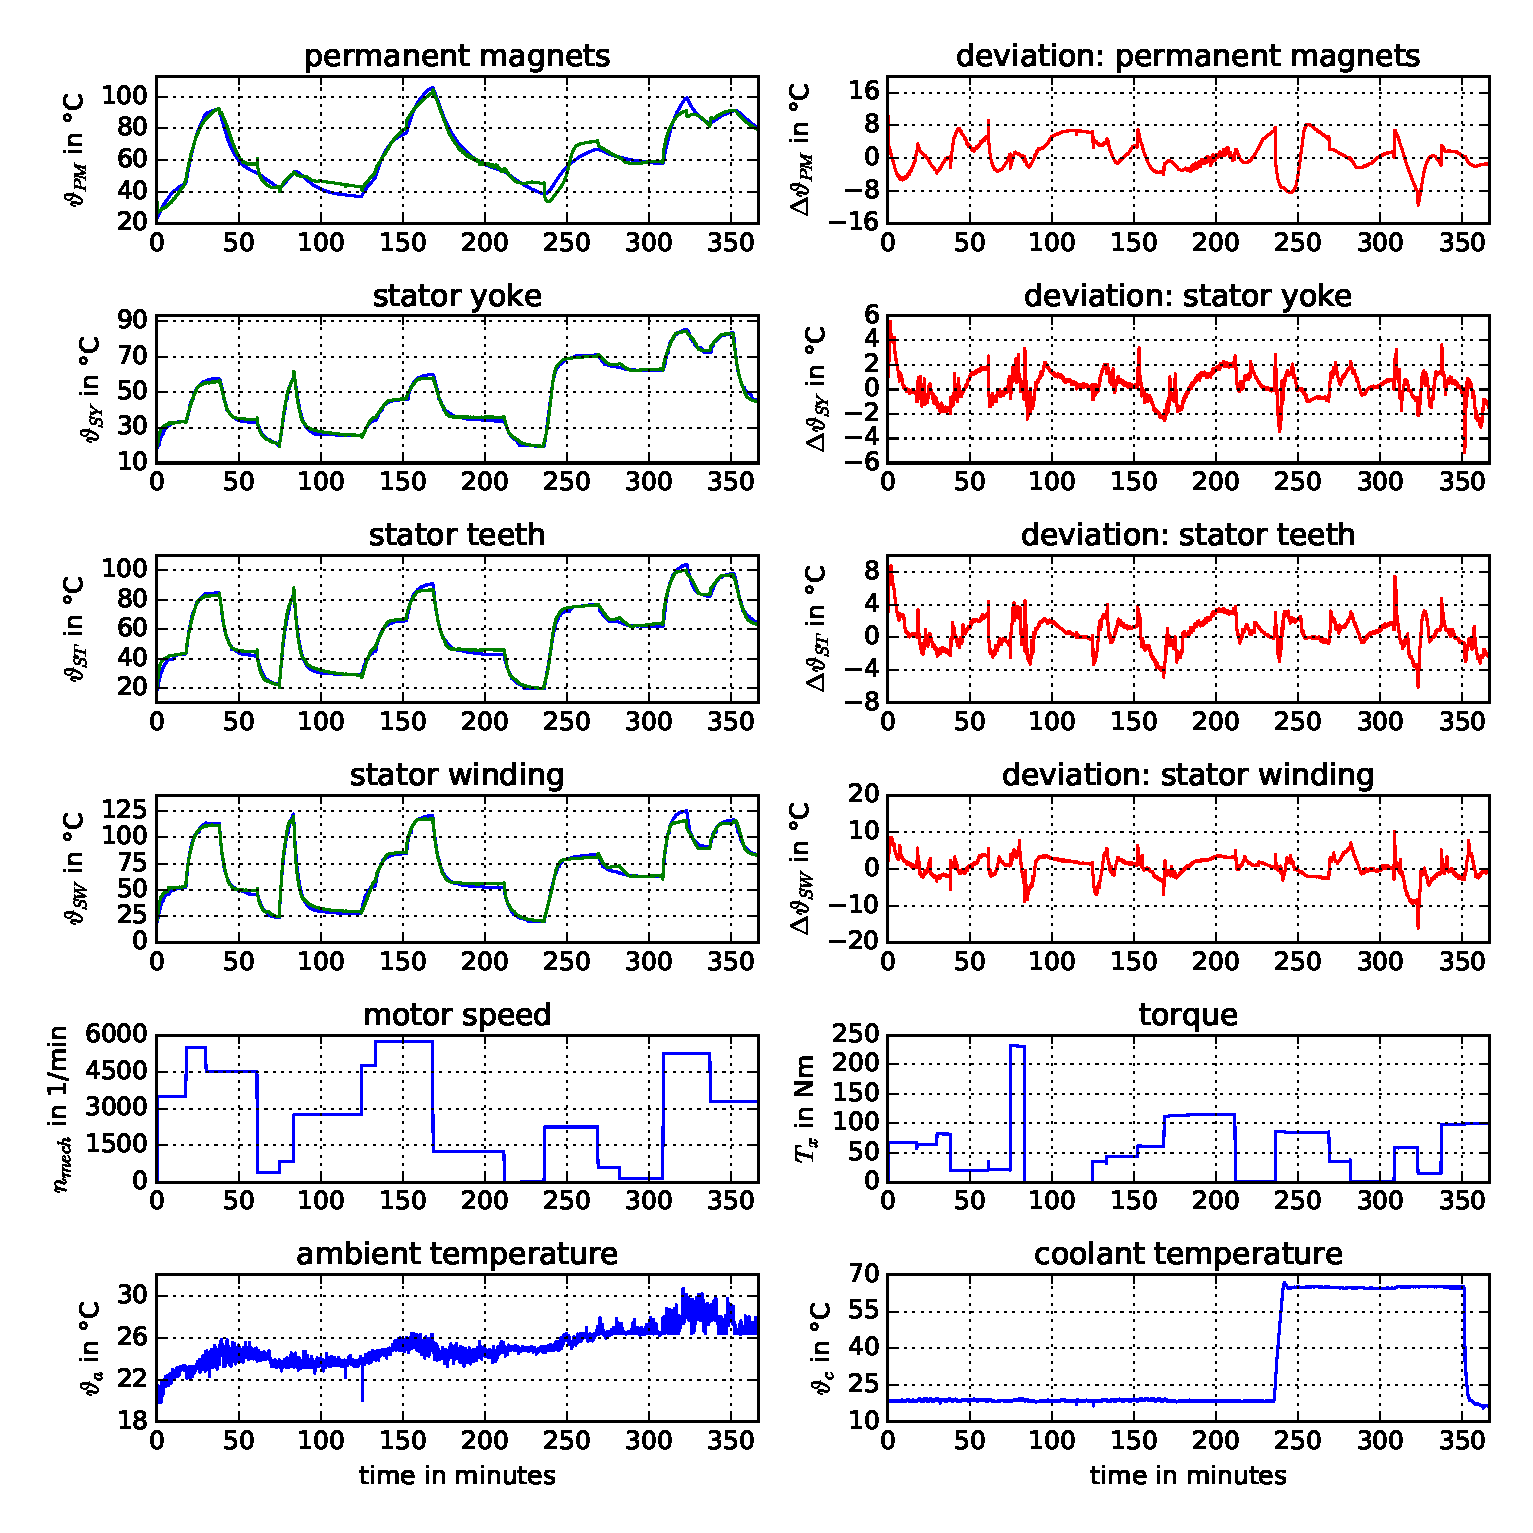
\includegraphics[width=\columnwidth]{evaluation/alltargets_test.eps}
	
	\caption{Cross-validation on the test subset (blue = measured groundtruth, green = prediction, red = deviation)}
	\label{fig:best_predictions}
\end{figure}

Here, the main finding from tab. \ref{tab:optimum_performance} is illustrated and confirmed again:
the permanent magnet temperature is obviously predicted poorly, while the stator temperatures were modeled decent.
One can infer from these plots, that neural networks seem to have trouble modeling the exponential rise and fall in the time series.
The largest distances between prediction and groundtruth happen when the prediction ceases following the exponential curves and stagnates to a plateau.

Comparing the prediction accuracy with those of \glspl{lptn} (see \cite{WaBo2016}), the achieved performance is similar, though during some time periods the worst-case deviation of permanent magnets and stator winding prediction dramatically exceeds that of \gls{lptn} estimates.

\subsection{Optimal Sets}
The particular choices of hyper-parameters for the optimum in each experiment are outlined in tab. \ref{tab:optimum_choices}.
\begin{sidewaystable}
	\caption{Hyper-parameter sets of the optima found in each experiment}
	\label{tab:optimum_choices}
	\centering\rarray{1.4}
	\begin{tabular}{c c c c c c c}
		\toprule
		 \quad & \multicolumn{6}{c}{experiment no.}\\
		 hyper-parameter & 1 & 2 & 3 & 4 & 5 & 6\\
		 \midrule
		 arch & \gls{lstm} & \gls{gru} & \gls{gru} & \gls{gru} & \gls{gru} & \gls{gru}\\
		 n\_hl & 1 & 1 & 1 & 1 & 1 & 1\\
		 n\_units & 35 & 122 & 143 & 236 & 115 & 38\\
		 weight init. distribution & unit normal & unit normal & unit normal & unit normal & unit normal & unit normal\\
		 weight init. scaling & normalized & normalized & normalized & standard & standard & normalized\\
		 seq\_len & 7800 & 7292 & 7880 & 862 & 360 & 6670\\
		 preprocess & standard & standard & standard & standard & standard & standard\\
		 pca\_var & 0.55 & 0.8 & 0.71 & 0.86 & 0.73 & 0.88\\
		 lookback & 937 & 822 & 2000 & 1060 & 880 & 732\\
		 opt & nesterov & adam & adam & adam & adam & adam\\
		 lr\_init & \num{1e-4} & 0.0172 & 0.0125 & 0.0112 & 0.0022 & 0.0217\\
		 lr\_decay & 0.98 & 0.97 & 0.95 & 0.9 & 0.79 & 0.66\\
		 active regularization & 3 & 1 & 1 & 2 & 2 & 2\\
		 gaussian noise & \num{1e-3} & \num{2.92e-5} & \num{1.54e-5} & \num{3.21e-4} & \num{3.82e-6} & \num{1.57e-4}\\
		 weight decay & \num{1e-4} & \num{7.23e-5} & \num{3.28e-5} & \num{1.55e-6} & \num{2.17e-6} & \num{2.22e-5}\\
		 \bottomrule
	\end{tabular}
\end{sidewaystable}

There are plenty of insights one can infer from the found optima.
First of all, homogeneously across all experiments, \gls{gru} with one hidden layer seems to be the optimal architecture; a unit normal weight initialization distribution appears being better than a uniform distribution; \gls{pca} is not improving performance over standard normalization and, as expected, Adam is the preferred optimizing technique.

The reason for \gls{gru} performing better than its counterparts might be its fewer adjustable weights, hence, it is less prone to over-fitting.
This thesis is further emphasized by the \gls{lstm} with peepholes having the worst scores and the highest number of weights to train.

The fact, that one hidden layer beats multiple might be due to the simplicity in the regression problem with respect to other problems in the real world, where deeper nets always perform better.
On the other hand, this optimum also might be caused by having too less training time allocated to the nets, though surveying the training trends for models with higher amounts of hidden layers reveals convergence most of the time.

Differences regarding the architecture are exhibited for the number of units.
Modeling the stator yoke demands a large amount of 236 units, while stator winding modeling requires mere 38 units.
This is a strong indicator for the different \gls{pso} durations, as shown in tab. \ref{tab:optimum_performance}.

Another interesting difference, especially between single target swarms, is evident in the subsequence lengths.
While permanent magnet temperatures need the maximum amount (7880 time steps) of comprehensive sequences, which suggests to drop the subsequences-strategy, stator winding temperatures can cope with around 6700 time steps and the other two stator temperatures are even satisfied with under 900 time steps, minimum at 360 time steps for experiment 5.
This evidences, that stator temperature regression in this particular task does benefit from the specially engineered subsequences-strategy, albeit this is not the case for the rotor temperature.

The necessity of long comprehensive sequences in case of permanent magnets becomes even more clear when examining the lookback optimum, which also points on the maximum length, whereby half of it suffices for stator temperatures.
As a reminder, saving statistical moments of certain time sequences poses infeasible memory requirements for automotive applications today.
Omitting these additional input quantities can be compensated by having more data as a basis for training.
Hence, the demand for long past sequences simultaneously constitutes the demand for more benchmark data.

The remaining differences in optimal hyper-parameter selection across the experiments are minor and their latent impact on performance is more thoroughly investigated in sec. \ref{sec:relevance}.

\subsection{Swarm Convergence}
Regarding the \glspl{pso}, sanity checks consisting of velocity monitoring and evaluation distribution as well as global best progress were executed.
Fig. \ref{fig:velocity} depicts how fast particles decelerate over all iterations upon the example of experiment 2.
Here, the mean absolute velocity of a particle is calculated by dividing the absolute velocity of each particle's dimension by the dimension's interval, summing all dimensions up and dividing again by the number of hyper-parameters, that is, by 15.
The velocity trend of the other experiments is very similar (see app. \ref{app:velocity}).

It becomes evident, that each swarm's particles slow down over time and converge to a certain spot in the search space.
This is the expected behavior since the velocity update formula has an expected mean at $E[c_{max}u] = 0.7$ for $c_{max} = 1.4$.  
% velocity convergence plot
\begin{figure}
	\centering
	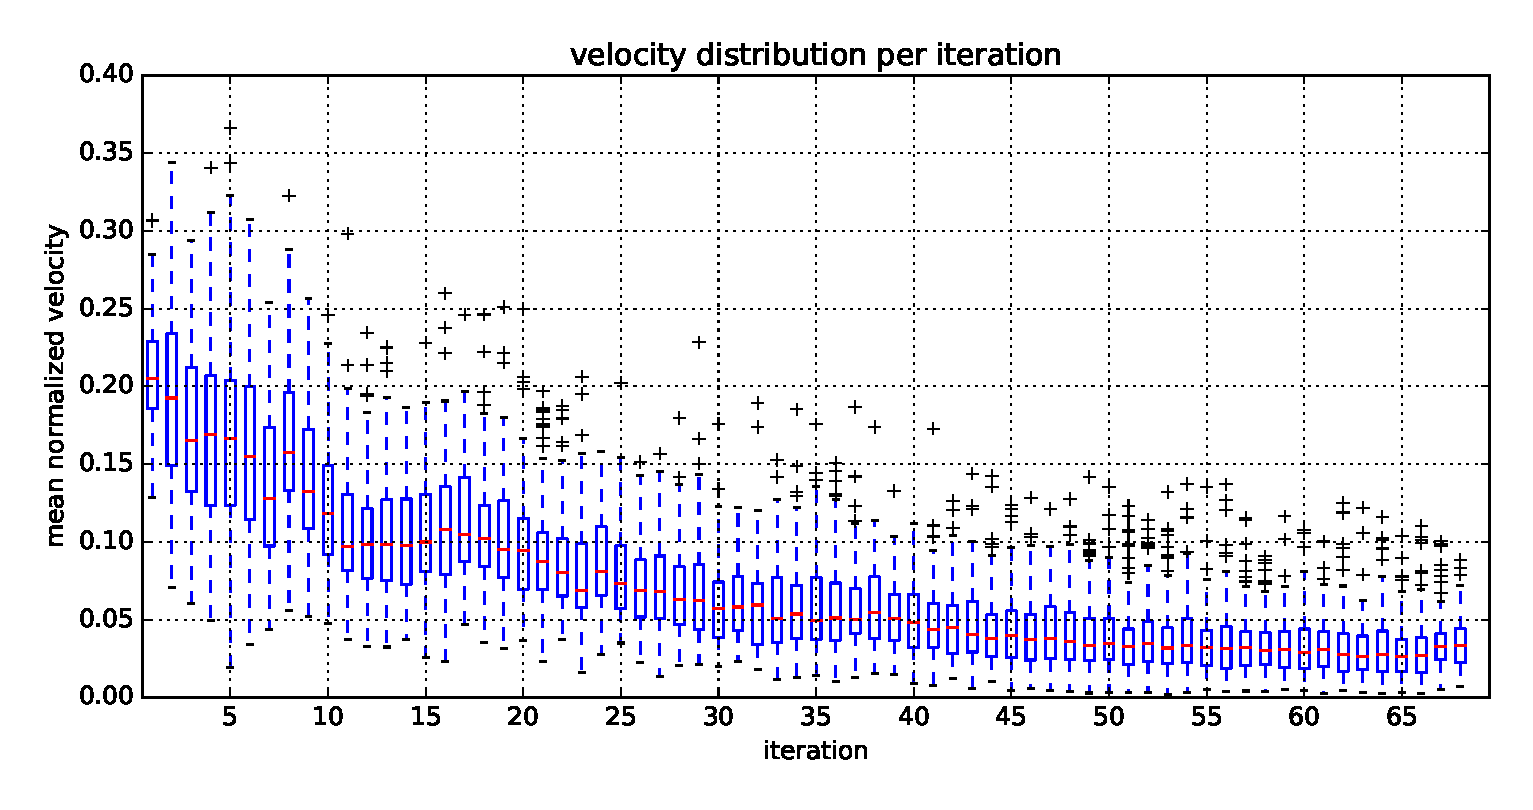
\includegraphics[width=\columnwidth]{evaluation/stator_vel.eps}
	\caption{Mean absolute velocity of the swarm's particles (from experiment 2)}
	\label{fig:velocity}
\end{figure}

% Evaluation distribution and gbest progress
In order to evaluate a swarm's performance, each particle's test score is displayed over the entirety of iterations in fig. \ref{fig:evaluation_development}, again, upon the example of experiment 2.
The global best progress is illustrated aside for better comparability.
The other experiments' trends show strong resemblance with fig. \ref{fig:evaluation_development} (see app. \ref{app:evaluation}).

% Describe what is seen in these plots
Fig. \ref{fig:evaluation_development} shows, that, up to a certain iteration, performance is not improving significantly anymore.
Moreover, the global best model is determined by lower outliers evaluated at apparently the same site in the search space.
This is indicated by the median of the particle test errors (the red mark) being at around the same performance level while the global best is still improving.
Assuming that as of the second half of iterations the same search space position's proximity is explored over and over again, one can infer from the broad scatter that the evaluation of a specific site comes with a broad variance as well.
\begin{figure}
	\centering
	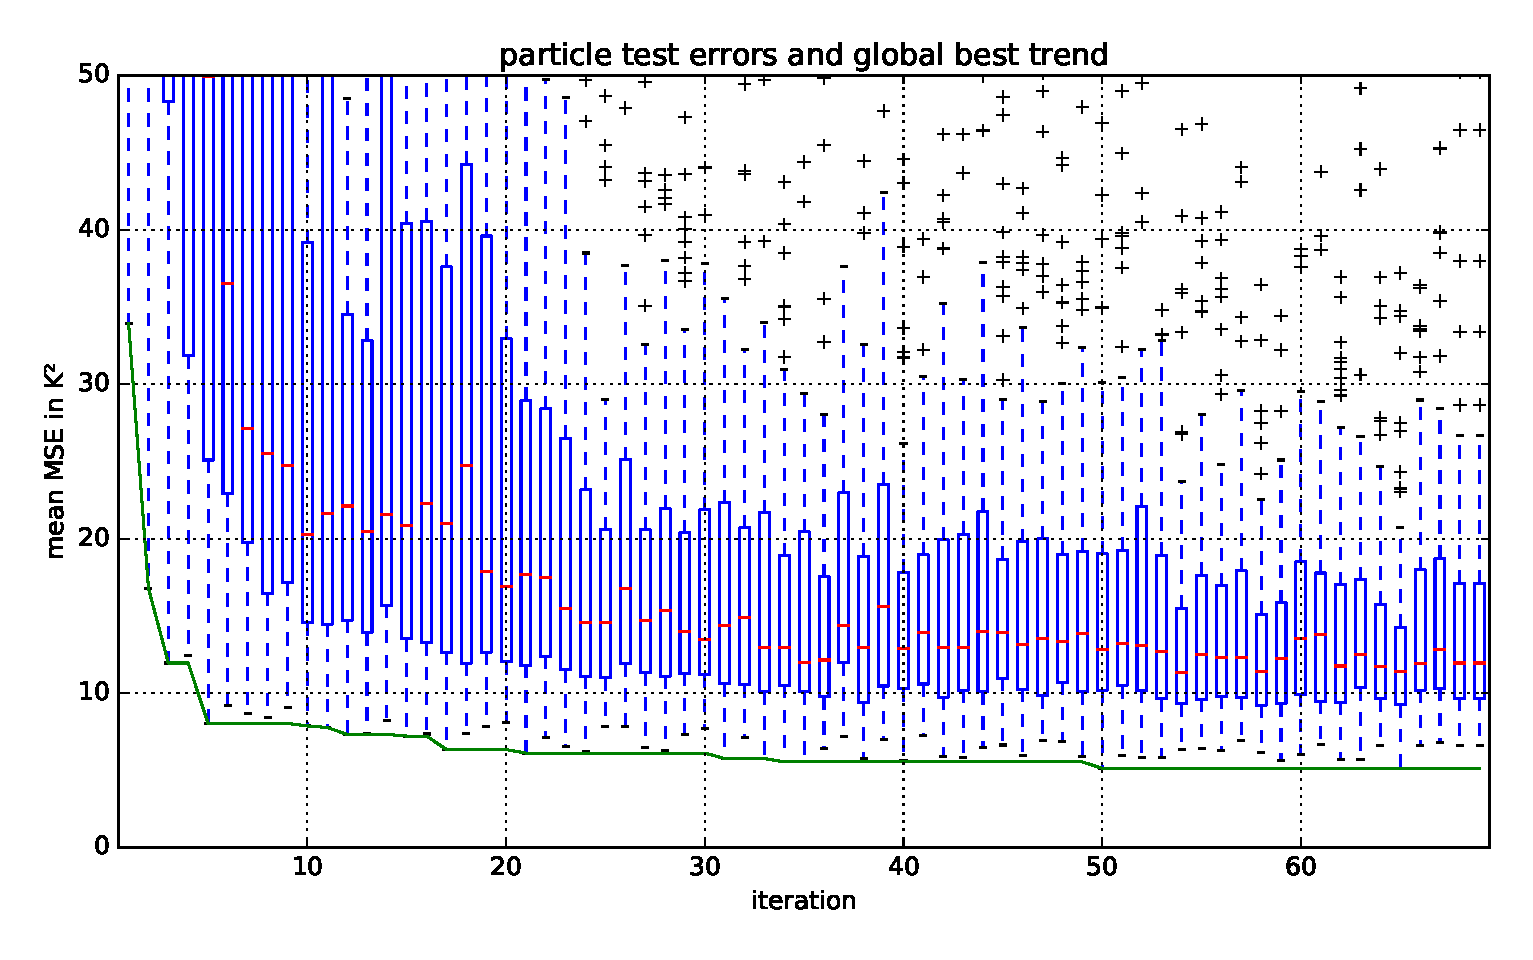
\includegraphics[width=\columnwidth]{evaluation/stator_eval.eps}
	\caption{Particle test scores over all iterations as box plots and the found best site's score as green line (from experiment 2)}
	\label{fig:evaluation_development}
\end{figure}

\subsection{Consistency}
In order to investigate the scatter of the optimal sites of each experiment, their optimal hyper-parameter sets were utilized for further 50 to 100 evaluations.
The resulting sample should give a clear insight to the mean performance and the standard deviation of the underlying hyper-parameters.

Fig. \ref{fig:consistency} depicts the scatter of the optimal hyper-parameters as histograms.
Outliers were removed, whereas an outlier is detected as such, if it has a score beyond 2.5 times the sample standard deviation.
Having outliers removed, a more robust sample standard deviation can be calculated.
The resulting sample means and standard deviations are stated in tab. \ref{tab:consistency}.

% consistency
%all targets: $\sigma = 4.55 K^2$. 15 samples zu $\pm 2.3 K^2$.
%stator: $\sigma=5 K^2$. 15 samples zu $\pm 2.53 K^2$.
%pm: $\sigma=13 K^2$. 73 samples zu $\pm 2.98 K^2$
%yoke: $\sigma=4.25$. 15 samples zu $\pm 2.15 K^2$.
%teeth: $\sigma=4.39$. 15 samples zu $\pm 2.22 K^2$.
%winding: $\sigma=5.57$ 15 samples zu $\pm 2.82 K ^2$.
\begin{figure}[!tbh]
	\centering
	\begin{subfigure}{0.31\textwidth}
		\includegraphics[width=\columnwidth]{evaluation/alltargets_consistency.eps}
		\caption{experiment 1 optimum}
	\end{subfigure}
	~
	\begin{subfigure}{0.31\textwidth}
		\includegraphics[width=\columnwidth]{evaluation/stator_consistency.eps}
		\caption{experiment 2 optimum}
	\end{subfigure}
	~
	\begin{subfigure}{0.31\textwidth}
		\includegraphics[width=\columnwidth]{evaluation/pm_consistency.eps}
		\caption{experiment 3 optimum}
	\end{subfigure}
	
	\begin{subfigure}{0.31\textwidth}
		\includegraphics[width=\columnwidth]{evaluation/yoke_consistency.eps}
		\caption{experiment 4 optimum}
	\end{subfigure}
	~
	\begin{subfigure}{0.31\textwidth}
		\includegraphics[width=\columnwidth]{evaluation/teeth_consistency.eps}
		\caption{experiment 5 optimum}
	\end{subfigure}
	~
	\begin{subfigure}{0.31\textwidth}
		\includegraphics[width=\columnwidth]{evaluation/winding_consistency.eps}
		\caption{experiment 6 optimum}
	\end{subfigure}
	\caption{Consistency tests showing histograms of the optimal hyper-parameters evaluated repetitively. Mean score of single-target experiments corresponds to the individual single target score.}
	\label{fig:consistency}
\end{figure}
\begin{table}[h]
	\caption{Sample characteristics for each consistency test}
	\label{tab:consistency}
	\centering
	\begin{tabular}{ c C{2cm} C{2cm} C{3cm} C{3cm}}
		\toprule
		 no. & $\mu$ (test)\quad in K\textsuperscript{2}& $\sigma$ (test)\quad in K\textsuperscript{2}&$\mu$ (validation)\quad in K\textsuperscript{2}& $\sigma$ (validation)\quad in K\textsuperscript{2}\\
		 \midrule
		 1& 33.16 & 4.54 & 48.07 & 2.39\\
		 2& 12.11 & 5.04 & 16.42 & 2.37\\
		 3& 38.41 & 13.02 & 56.42 & 8.19\\
		 4& 7.8 & 4.25 & 9.1 & 1.03\\
		 5& 12.41 & 4.39 & 24.51 & 2.57\\
		 6& 21.53 & 5.57 & 38.41 & 4.08\\
		  \bottomrule
	\end{tabular}
\end{table}

It becomes clear from fig. \ref{fig:consistency} and tab. \ref{tab:consistency}, that there is a large scatter inherent in every search space site's evaluation and that the best performances are critical outliers of that specific position.
Although the hyper-parameters are set constant, the evaluation on the test set cannot be stated unambiguously by a mere single evaluation, as it was conducted during this work's experiments, but rather by the mean of multiple evaluations, that would vary within a certain significance interval to a given chance (usually 95\,\%).
For instance, assuming the standard deviation estimate from the consistency tests represents the true standard deviation sufficiently, one would have to execute 15 evaluations of a single spot in order to be able to declare this sample's mean to be in an interval length of under 6\,K\textsuperscript{2} with a 95\,\% chance.
This is the case for all experiments except for experiment 3, which has its standard deviation estimate at around 13\,K\textsuperscript{2} instead of approx. 5\,K\textsuperscript{2}.
Unfortunately, that would also mean to have the experiment duration increased fifteenfold, which slingshots the \gls{pso} to infeasibility.
In case of experiment 3, even 73 evaluations were required.

The reason for the large scatter is undoubtedly rooted in the random weight initialization since gradient descent training is very sensitive to its initial starting point in the error landscape.
One could go ahead and set a constant seed to the random number generators, but that would only ensure reproducibility and the investigation's exploratory character were sapped.

However, facing these facts, the found optima cannot be declared reliably best in terms of performing best on the test set on average, yet they surely are close to optimal sets as numerous particles were tempted to find a global optimum.
Furthermore, the obtained results give a fair insight to what extent neural networks are capable of modeling important component temperatures inside \glspl{pmsm}.

\section{Hyper-Parameter Relevance}
\label{sec:relevance}
Having determined close to optimal hyper-parameters for each target, one is interested in how far each hyper-parameter is important for a decent modeling.
If it is possible to track those parameters having no impact on the modeling performance, then future investigations could concentrate on less or other input measures.

\subsection{Scatter Over PSO Iterations}
% parameter distribution
Before an extensive sensitivity analysis is conducted, the specific choice of hyper-parameters over all iterations are investigated first.
Since the coarse global optimum site in the search space is presumably found early on, most of the choices should be distributed on the optimal choices.
Hyper-parameters, which are more or less uniformly distributed over their full interval, were likely changing their global best value frequently together with the global optimum progress.
This indicates, that those hyper-parameters were not of much relevance, since completely different values were found to be the very best more often.
Conversely, if a hyper-parameter is distributed narrowly around a certain value, then this value was probably found to be the best relatively early without fail during later transitions of the global optimum.

Fig. \ref{fig:param_dist} presents the distribution of all hyper-parameters over the entirety of iterations in experiment 4.
The remaining distribution plots are attached to app. \ref{app:param_dist}.
\begin{figure}[!bth]
	\centering
	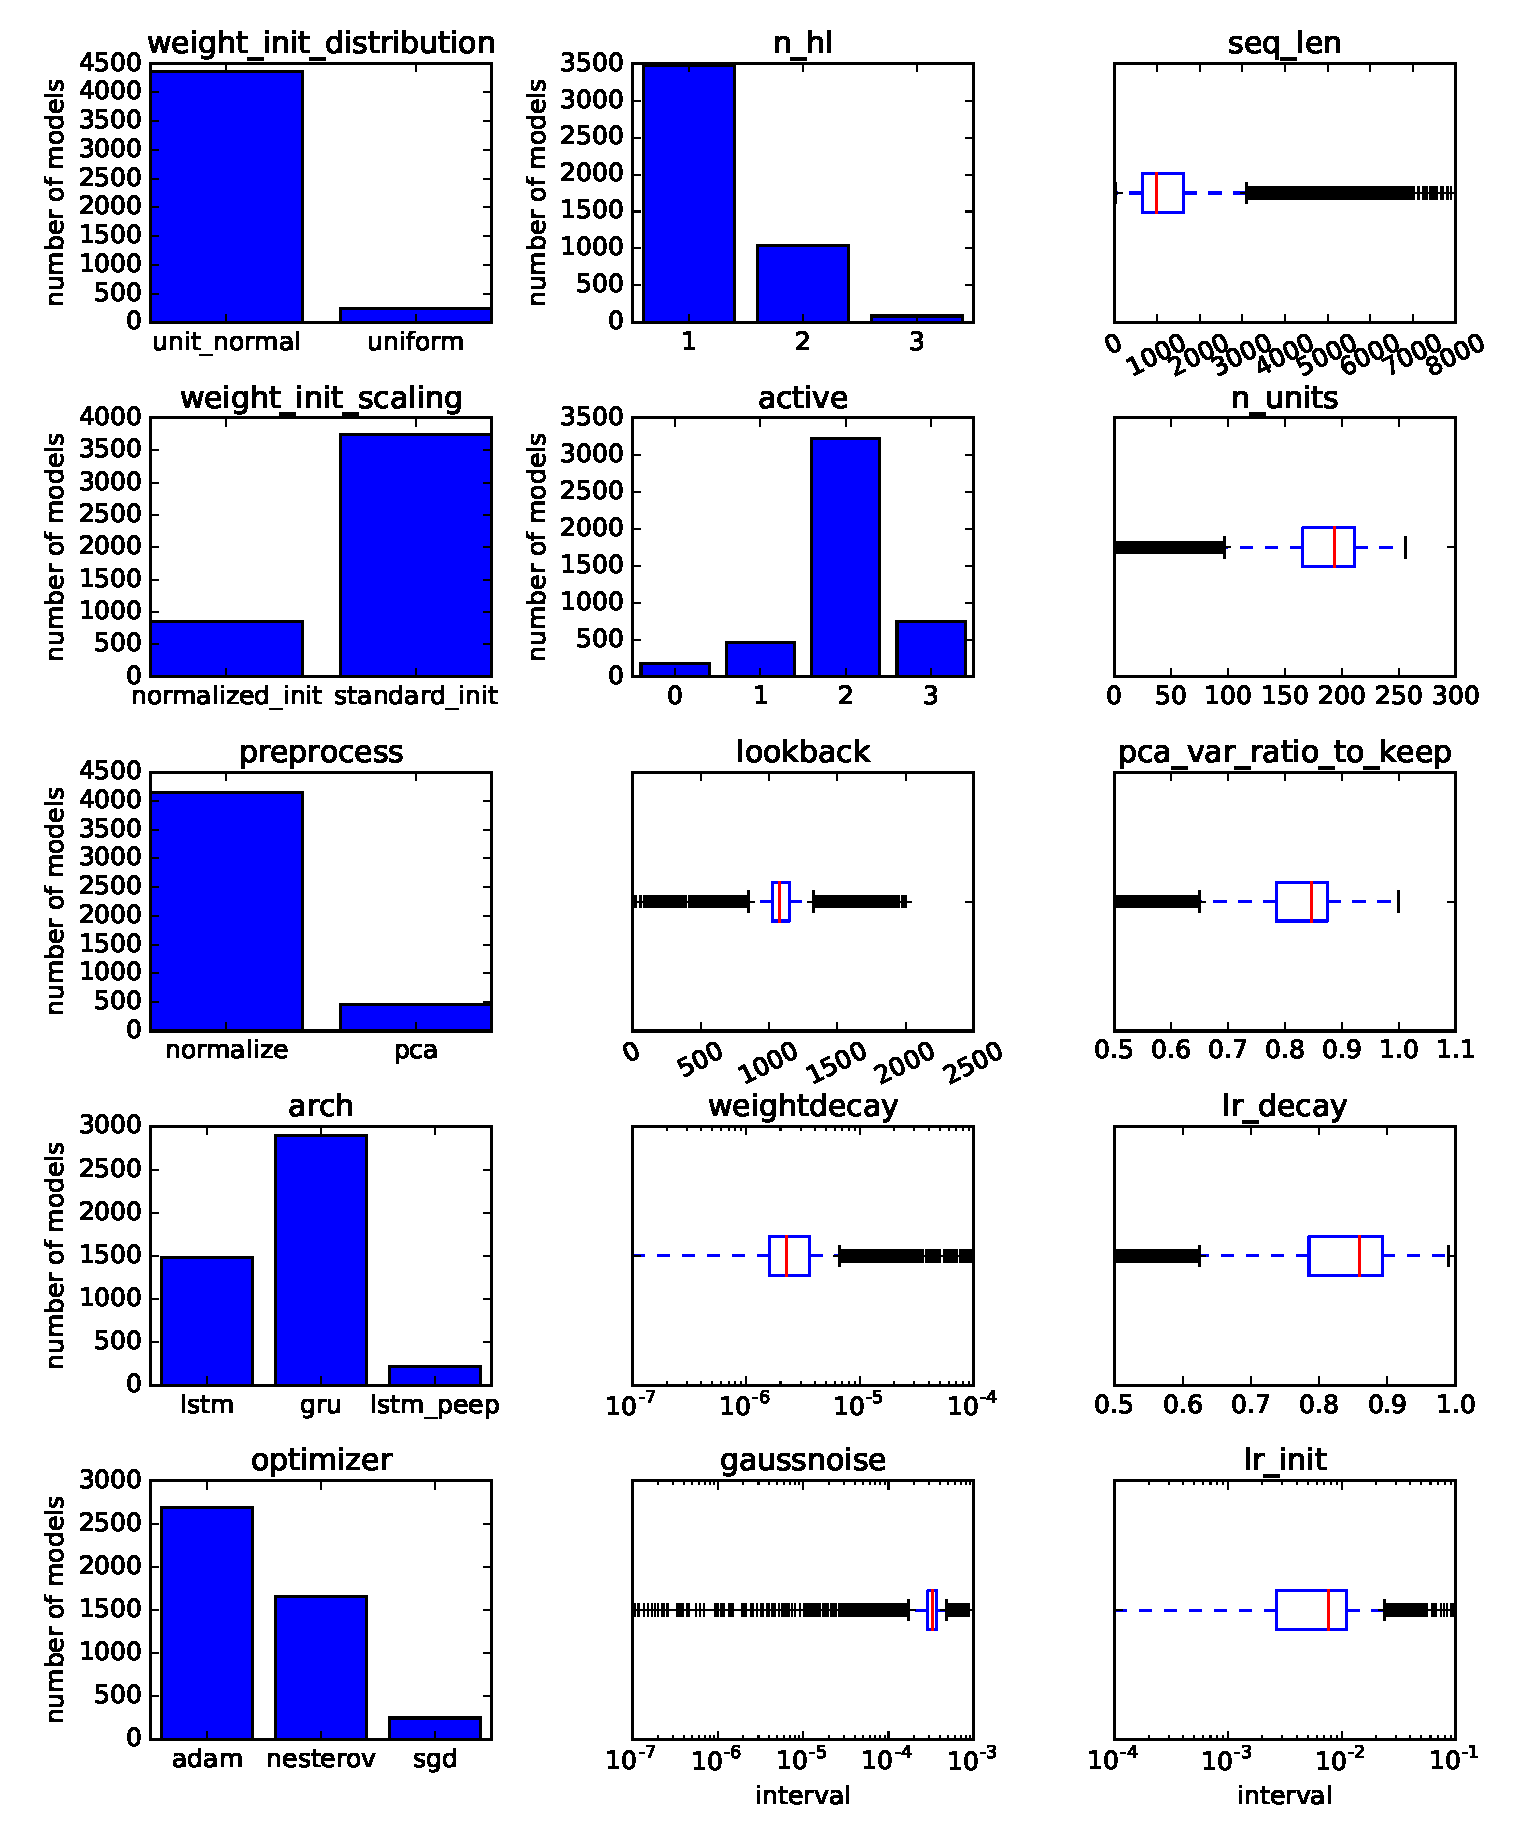
\includegraphics[width=\columnwidth]{evaluation/yoke_paramdist.eps}
	\caption{Bar plots and box plots depicting the distribution of each hyper-parameter over all \gls{pso} iterations (from experiment 4)}
	\label{fig:param_dist}
\end{figure}

Comparing the distributions in fig. \ref{fig:param_dist} with the optimal values of experiment 4 in tab. \ref{tab:optimum_choices}, it becomes clear, that the vast bulk of choices are indeed set around the optimum.
The same situation is observable for the other distribution plots in app. \ref{app:param_dist}.
This hint underlines the thesis, that during the whole \gls{pso}, the global best site's proximity is more thoroughly explored than other sites.

Now for the very case of experiment 4, it becomes evident, that some parameter distributions are more spiked around the optimum than others.
The lookback value, for instance, is relatively narrowly distributed, while learn rate decay or number of units is scattered broadly.
This might give a clue about their relevance, as narrowly distributed parameters could tend to exhibit higher sensitivity with respect to model performance than those being flat on the interval.

To summarize what can be found across the board, it can be reliably stated, that obviously concentrated and simultaneously identical distributions are presented by the weight initialization distribution, number of hidden layers, preprocessing variant and architecture.
Regarding the optimizer technique, the stator-yoke-targeted model is the only one, which holds a respectable amount of choices for Nesterov next to \gls{adam}, while all other experiments are almost exclusively attracted to Adam. 
The weight initialization scaling and lookback are also in a peaked shape, but various across experiments.
The other hyper-parameters are widely spread over their interval for at least one experiment.

Unfortunately, there is nothing, that can be inferred from the \gls{pca} variance hyper-parameter distribution as it is practically never applied according to the preprocess hyper-parameter, which sticks to all-standard normalization rather than \gls{pca}.

In order to complement the findings from the parameter distribution plots, the unit interval variances of each hyper-parameter over \gls{pso} iterations are illustrated as well.
Fig. \ref{fig:param_var} depicts that trend for experiment 4.
Hyper-parameters with few alternatives are drawn with solid lines, while the rest is assigned dashed lines.
Those hyper-parameters with a logarithmic scale (see distribution plots) have their unit variance evaluated on the logarithmic scale either.
The hyper-parameter unit interval variances plots for the remaining experiments are attached to app. \ref{app:param_var}.

\begin{figure}[!tbh]
	\centering
	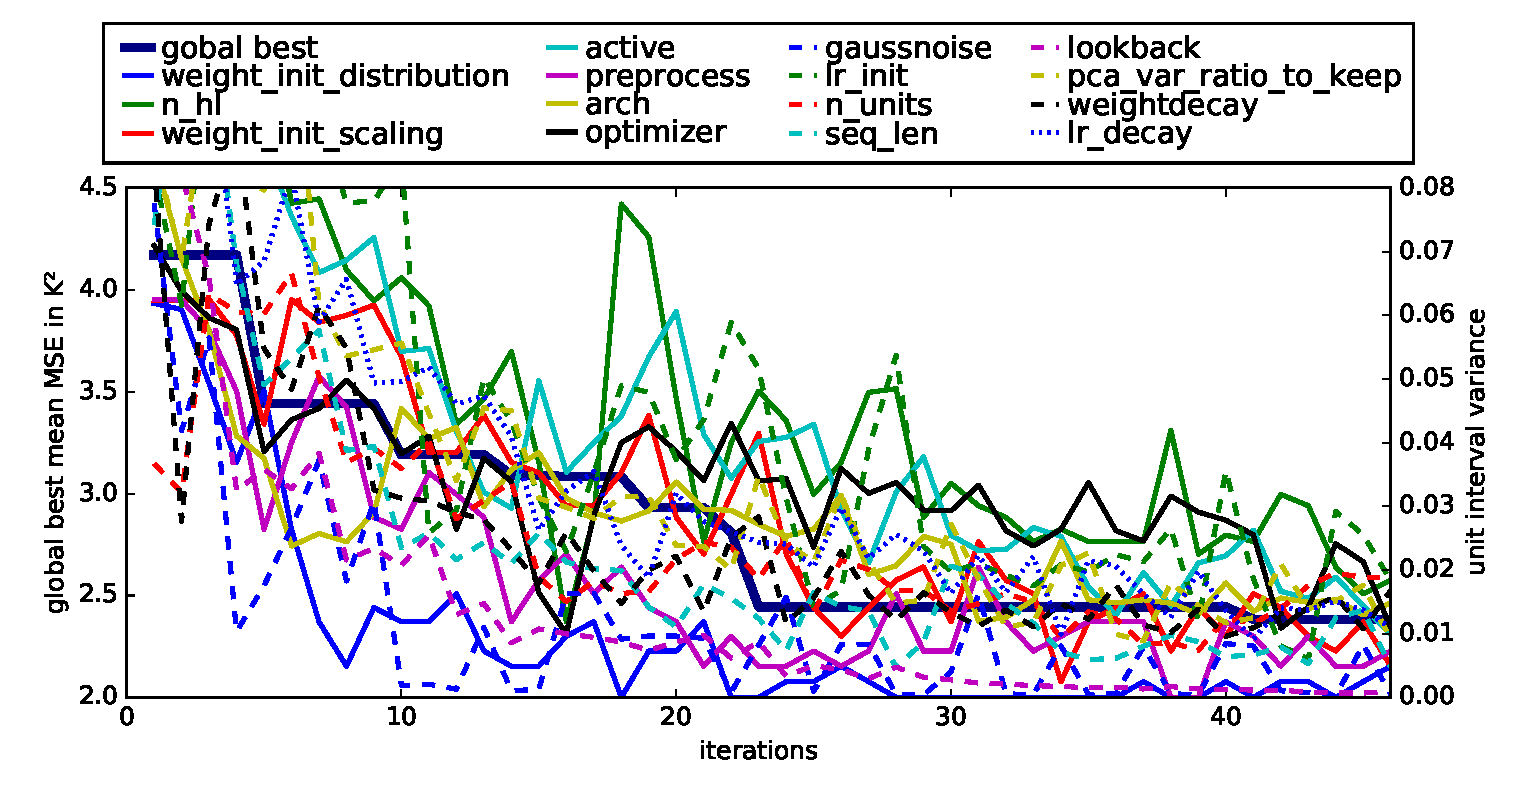
\includegraphics[width=\textwidth]{evaluation/yoke_var.eps}
	\caption{Hyper-parameter variance over \gls{pso} iterations (from experiment 4)}
	\label{fig:param_var}
\end{figure}

One can infer from the variance trends, that those hyper-parameters, that are of a peaked shape in the distribution plots, also show low variance during most of the \gls{pso} iterations.
Consequently, if narrowly distributed parameters inherit high relevance for model performance, it is plausible for them to have a low variance early on or in the progress of the \gls{pso}.
A high sensitivity of the model to low-varying hyper-parameters would be the conclusion, which is to be proven in the next subsection.
Note, that the unit variances calculated here heavily depend on the predefined interval, in which the hyper-parameter was moving.
It is also worth mentioning, that regularization techniques' variance or \gls{pca} variance trends are difficult to interpret, as their corresponding activation parameters ( `active' and `preprocess') were likely to cut them off.

Fig. \ref{fig:param_var} suggests, that for the case of experiment 4 the parameters `lookback', `preprocessing', `gaussian noise' and `weight init. distribution' hold most of the relevance, while `number of hidden layers', `optimizer' and `learn rate init.' go without much impact on model performance, which can be confirmed by the distribution plot in fig. \ref{fig:param_dist}.
Yet, the finding for `gaussian noise' is misleading, because it was seldom applied according to fig. \ref{fig:param_dist}, thus, there was rather a pseudo-relevance formed during the \gls{pso}.


\subsection{Sensitivity Analysis}
In order to obtain a deeper sense for the hyper-parameters' relevance in terms of sensitivity with respect to model performance, a sensitivity analysis is conducted for the optimum found in each experiment.

The strategy during the sensitivity analysis is as follows:
for hyper-parameters, that have a continuous interval, evaluate alternatives of $\pm$ 10\,\% of that interval, or, if this would exceed an interval bound, select that bound instead.
If the optimum lays on the upper or lower bound, then evaluate just the valid alternative laying within the interval.
For hyper-parameters with mutually exclusive choices, evaluate all alternatives other than the optimum.
In case of preprocessing, if the optimum is standard normalization (which is the case for all experiments), then evaluate a model with \gls{pca} as preprocessing and a variance to keep of 50\,\% and 100\,\% each.
In case of active (regularization), evaluate models with all alternative combinations, where standard deviation of gaussian gradient noise, respectively, the weight decay factor is set default to \num{1e-6}.

For experiments 1, 2, 4, 5 and 6 there are 15 models conducted for each alternative, while for experiment 3 the sample consists of 73 \glspl{ann}.
The sample mean of each alternative represents the estimated performance of that particular hyper-parameter set.
A 95\,\% confidence interval is given for each experiment's analysis, assuming the alternatives inherit the same standard deviation as the optimum.
The varying performance is compared upon the test score.
For each experiment, the baseline is given by the sample characteristics found during the consistency tests (see tab. \ref{tab:consistency}).

Tab. \ref{tab:sensitivity} exemplifies the outcome of the sensitivity analyses upon experiment 4.
Again, the remaining tables are attached to the appendix (see app. \ref{app:sensitivity}).

\begin{table}[h]
	\caption{Sensitivity analysis for experiment 4}
	\label{tab:sensitivity}
	\centering
	\begin{tabular}{ C{2.5cm} C{2.5cm} c c}
		\toprule
		\multicolumn{2}{c}{optimum: \SI{7.8}{\kelvin\squared}}&\multicolumn{2}{c}{95\,\% confidence interval: $\pm$ 2.15\,K\textsuperscript{2}}\\
		\midrule
		 hyper-parameter & alternatives & test score estimates in K\textsuperscript{2} & $\Delta$ w.r.t. baseline in K\textsuperscript{2}\\
		 \midrule
		 arch				& \gls{lstm}/ \gls{lstm}+peepholes& 28.17/ 265.32 		& 20.37/ 257.52 \\
		 n\_hl				& 2 							& 98.57 				& 90.77 \\
		 n\_units				& 142/ 300					& 6.86/ 17.64 			& -0.94/ 9.84 \\
		 opt					& nesterov/ \gls{sgd} 			& 14.79/ 8.95 			& 6.99/ 1.15  \\
		 seq\_len				& 77/ 1647 					& 12.38/ 29.35 		& 4.58/ 21.55\\
		 lookback				& 860/ 1260 					& 7.36/ 6.3	 		& -0.44/ -1.5\\
		 lr\_init				&\num{5.65e-3}/ \num{2.25e-2}	& 6.78/ 103.95			& -1.02/ 96.15\\
		 lr\_decay 			& 0.85/ 0.95					& 6.17/ 5.75			& -1.63/ -2.05\\
		 preprocess 			& \gls{pca}: 0.5/ 1.0				& 353.53/ 81.3			& 345.73/ 73.5\\
		 weight init. distribution& uniform					& inf.				& inf.\\
		 weight init. scaling 	& normalized 					& 49.18 				& 41.38\\
		 active 				& 0/ 1/ 3						& 5.64/ 15.10/ 7.84		& -2.16/ 7.3/ 0.04\\
		  \bottomrule
	\end{tabular}
\end{table}

The sensitivity analysis reveals in how far model performance deviates when single hyper-parameters are varied slightly.
For mutually exclusive choices in hyper-parameters, this variation may turn out more severe, as they do not consist of continuous intervals, and their alternatives are not measurable in a $\pm$ 10\,\% fashion.

However, what can be inferred from tab. \ref{tab:sensitivity} explicitly is the fact, that altering hyper-parameters like `weight init. distribution and scaling', `preprocessing' and number of hidden layers (`n\_hl') has a large negative impact on the model's test score.
This shapes up to be in concert with the findings in the previous subsection, except for `n\_hl', which has shown large variance in the variance trend throughout the \gls{pso} but now proves essential for model performance.
Conversely, `lookback' was predicted important upon surveying the variance trend and now shows to be particularly insignificant around its optimal selection.
Furthermore, architecture plays a big role regarding one of both alternatives, namely, when selecting \gls{lstm}+peepholes, which devastates prediction accuracy, whereby it showed modest variance, which is probably due to the lower influence by the other alternative (plain \gls{lstm}).
Similar to the architecture, learn rate init. has a low significance upon reduction but exhibits the more seismic when being increased.
The reason for this is clearly rooted in the gradient descent technique, that starts oscillating around local optima when being initialized with a too high learn rate factor.
The considered \glspl{ann} seem to be especially robust around the optimum selection with respect to changes in the parameters `lookback', `optimizer', `number of units', `learn rate decay' and varying regularization techniques, which also has shown moderate variances in fig. \ref{fig:param_var}.

Note, that the infinity score for the weight init. distribution alternative is due to the activation functions inside the neurons having to divide extraordinarily small values and, eventually, having to divide zero by zero, which leads to a `NaN' outcome (the chainer framework supports 32-bit float precision to this date only).
This situation is indeed not unusual, especially in the \gls{pso} environment and its first iterations, where unfavorable parameter combinations are forced together in an exploratory way.
This explains, why particles refrained from selecting the uniform distribution, as this obviously resulted in enormously high test errors for the most of appropriate hyper-parameters for the optimum distribution.  

While most of the findings here accord with those in the parameter distribution and variance trend plots, some hyper-parameters do not show the expected sensitivity as suggested by the previous subsection.
The cause for this might lay in the different procedures conducted for the \gls{pso} and for the sensitivity analysis.
As mentioned before, the \gls{pso} was evaluating each spot in the search space just once and pursued the very next better test score of each site, instead of rating a spot according to its average evaluation calculated from a sample (which would have been infeasible).
Yet some hyper-parameters, when kept constant, may result in more test score scatter than others.

This theory applied to the case of `number of hidden layers' in experiment 4:
tab. \ref{tab:sensitivity} proves, that altering number of hidden layers to two would result in a much worse test score \textit{on average}, although particles tended to vary that parameter eagerly according to fig. \ref{fig:param_var} .
If the test score of several samples of that alternative shows a large variance now, then there also might be a certain amount of decent results for a two layered neural network, which were often unluckily detected by many particles.
This emphasizes the importance of a sensitivity analysis as a complementary investigation to parameter scatter over \gls{pso} iterations.  

The discrepancy between the \gls{pso} objective and sensitivity analysis objective becomes even more evident, as some alternatives for some experiments show even better average test scores than the optimum's average test score (which are stated in tab. \ref{tab:consistency}).
The improvements are relatively minor, but in case of experiment 3 and hyper-parameter `sequence length' it is especially obvious with an improvement of \SI{-8.21}{\kelvin\squared} on average.
It even turned out, that one of the 73 models representing the sample for the `sequence length'-alternative at 7095 time steps has beaten the optimum by \SI{2.87}{\kelvin\squared} with a test score of \SI{10.68}{\kelvin\squared}.

In summary, following can be concluded for the hyper-parameters' relevance in this thesis' particular modeling task:
\begin{itemize}
	\item \gls{gru} beats both, \gls{lstm} and even more \gls{lstm}+peepholes, in almost every case,
	\item small networks with one hidden layer perform in this particular setup clearly better than deep networks,
	\item Adam as optimizer technique outplays Nesterov-style momentum training and classic \gls{sgd}, whereby this is not significant when modeling stator temperatures,
	\item too large learn rate initializations can stop training, but too small values do not harm performance heavily (yet it can prolong training time),
	\item preprocessing the data with a \gls{pca} is no good and should be avoided in any case,
	\item assigning a uniform random disribution to the weight initialization often leads to numerical problems and should also be avoided,
	\item the wrong weight init. scaling can harm performance but which is wrong depends on the model's target and should be investigated independently, as well as
	\item sequence length exhibits slight sensitivity but the optimal range is polarized through its interval bounds by different experiments and
	\item the remaining hyper-parameters (number of units, lookback, learn rate decay and the regularization techniques) show mixed but minor relevance to the model performance. Thus, they can be set constant to an appropriate range and may be neglected for further hyper-parameter optimizations. 
Other hyper-parameters, which are not considered here, may come into play instead.
\end{itemize}

\section{Model Ensembles}
It is a well known fact, that averaging the prediction of multiple models for a certain task improves precision slightly without any other effort.
Grouping these models together to a new model, whose prediction results from the individual models' prediction average, one obtains a \textit{model ensemble}.

In an attempt to investigate the possible chances offered by model ensembles, several best performing neural networks from each experiment are combined ad hoc.
Usually, it is recommended to ensemble diverse models rather than the same model holding varying, trained parameters, as different model structures may also learn different latent patterns from the input data.
Utilizing the diversity in a model ensemble to achieve better results by overcoming the drawbacks of individual model families is the intention here. 
However, since in this work \glspl{ann} were trained exclusively, they represent the only source to draw ensemble-members from.

The particular strategy was as follows:
Consider the 20 best performing models for each experiment and evaluate the mean in a cumulative manner, that is, average the best two models first, then the best three models, the best four and so on.
From each experiment, the best of 19 model ensemble performances with their improvement with respect to the optimum found in the \gls{pso} is stated in tab. \ref{tab:ensemble}
%model ensemble chances

\begin{table}
	\caption{Model ensembles}
	\label{tab:ensemble}
	\centering\rarray{1.4}
	\begin{tabular}{ c C{1.7cm} C{1.7cm} C{2.5cm} C{2.5cm} C{2.5cm}}
		\toprule
		 experiment & ensemble size & \multicolumn{2}{c}{MSE} & \multicolumn{2}{c}{deviation}\\
		 \quad & \quad & test score in K\textsuperscript{2} & $\Delta$ w.r.t. baseline in \si{\kelvin\squared} & max. dev. in \si{\celsius} & $\Delta$ w.r.t. baseline in \si{\kelvin\squared}\\
		 \midrule
		 1		& 2 		& 23.85	& -0.65 & $\vartheta_{PM}$: 28.83/ $\vartheta_{SY}$: 10.79/ $\vartheta_{ST}$: 17.19/ $\vartheta_{SW}$: 37.48 & 10.18/\qquad 5.24/\qquad 8.39/\qquad 18.36\\
		 2		& 9		& 3.95 	& -1.15 & $\vartheta_{SY}$: 9.37/ $\vartheta_{ST}$: 14.13/ $\vartheta_{SW}$: 18.71 & 3.82/\qquad 5.33/\qquad -0.39 \\
		 3		& 9		& 9.97 	& -3.58 & 16.31& -1.84 \\
		 4		& 6		& 1.75	& -0.63 & 7.56 & 2.01 \\
		 5		& 18		& 4.59	& -0.9 & 13.76 & 4.97 \\
		 6		& 5 		& 8.02 	& -1.41 & 20.09 & 0.97\\
		  \bottomrule
	\end{tabular}
\end{table}
%exp3. pm
%max. dev for permanent magnets: 18.14587696242438 °C
% exp2. stator
%max. dev for stator yoke: 5.552190350208548 °C
%max. dev for stator teeth: 8.795146986444024 °C
%max. dev for stator winding: 19.123281519553416 °C

It becomes obvious, that even with a simple ensemble strategy, as it is conducted here, improvements in the mean squared error are possible.
Although they are minor, this demonstrates, that model ensembles are an effective method to gain slightly better performance from a set of trained models.
Though most of the depicted ensembles hold a larger maximum deviation, there are often ensembles among the 19 conducted, that have a slightly worse test score but therefore a much smaller maximum deviation.
However, for experiment 5, there is no significantly better maximum deviation within the ensembles.
Finding a reasonable compromise will be desirable.
Note, that the ensemble members for the single-targeted models (experiment 3-6) are exclusively selected from there as well, but compared upon the very best predictions, which for experiment 4-6 originate from experiment 2.
The individual targets' maximum deviation in experiment 1 and 2 are also compared upon the best found solutions in experiment 2 and 3.

It is further worth mentioning, that model ensembles multiply computational requirements, which might prove infeasible in certain fields of application.

For experiment 2, the model ensemble's individual target scores (not displayed in the table) again exhibit the very best mean squared error of stator temperature predictions with \SI{1.71}{\kelvin\squared}, \SI{3.17}{\kelvin\squared} and \SI{6.95}{\kelvin\squared} for the stator yoke, teeth and winding, respectively.

More sophisticated ensemble algorithms may take a weighted average from the ensemble members, where better models are assigned more weight.
Another alternative would be to survey which models tend to overestimate the groundtruth and which underestimate it on average, such that they are mixed in equal shares.
A full-size adaptive parameter optimization could be conducted solely for the optimal combination of models.
The possibilities are endless.

